\documentclass[12pt]{article}
\usepackage[utf8]{inputenc}
\usepackage[T1]{fontenc}
\usepackage{graphicx}
\usepackage[export]{adjustbox}
\graphicspath{ {./images/} }
\usepackage{amsmath}
\usepackage{amsfonts}
\usepackage{amssymb}
\usepackage{amsthm}
\usepackage[version=4]{mhchem}
\usepackage{stmaryrd}
\usepackage{hyperref}
\hypersetup{colorlinks=true, linkcolor=blue, filecolor=magenta, urlcolor=cyan,}
\urlstyle{same}
\usepackage[margin=1in]{geometry}
\usepackage{titlesec}
\usepackage{appendix}

\usepackage{parskip}
%\setlength{\parskip}{0pt} % 1ex plus 0.5ex minus 0.2ex}
%\setlength{\parindent}{0pt}

\usepackage{setspace}
\setstretch{1.5}
\renewcommand{\arraystretch}{1}
\titlespacing{\section} {0pt}{2ex}{2ex}

\newtheorem{theorem}{Theorem}[section]
\newtheorem{proposition}{Proposition}[section]

\theoremstyle{definition}
\newtheorem{example}{Example}[section]
\AtEndEnvironment{example}{\null\hfill\qedsymbol}

\renewcommand{\thefigure}{\arabic{section}.\arabic{figure}}

\title{ECON 2080: Continuous Time\\Spring 2024}


\author{Fernando Duarte\thanks{Brown University}}
\date{}


%New command to display footnote whose markers will always be hidden
\let\svthefootnote\thefootnote
\newcommand\blfootnotetext[1]{%
  \let\thefootnote\relax\footnote{#1}%
  \addtocounter{footnote}{-1}%
  \let\thefootnote\svthefootnote%
}

%Overriding the \footnotetext command to hide the marker if its value is `0`
\let\svfootnotetext\footnotetext
\renewcommand\footnotetext[2][?]{%
  \if\relax#1\relax%
    \ifnum\value{footnote}=0\blfootnotetext{#2}\else\svfootnotetext{#2}\fi%
  \else%
    \if?#1\ifnum\value{footnote}=0\blfootnotetext{#2}\else\svfootnotetext{#2}\fi%
    \else\svfootnotetext[#1]{#2}\fi%
  \fi
}

\begin{document}
\maketitle


\section{Brownian Motion}
Brownian motion is a continuous-time scalar stochastic process such that, given the initial value $x_{0}$ at time $t=0$, the random variable $x_{t}$ for any $t>0$ is normally distributed with mean $\left(x_{0}+\mu t\right)$ and variance $\left(\sigma^{2} t\right)$. The parameter $\mu$ measures the trend, and $\sigma$ the volatility, of the process. This process was first formulated to represent the motion of small particles suspended in a liquid. We shall sometimes refer to a ``particle'' performing the Brownian motion, $x_{t}$ as its ``position'', and a graph of $x_{t}$ against $t$ as its ``path''.

We can think of Brownian motion as the cumulation of independent identically normally distributed increments, the infinitesimal random increment $dx$ over the infinitesimal time $dt$ having mean $\mu dt$ and variance $\sigma^{2} dt$. Just as we would write a general normal $(\mu, \sigma)$ variable as $\mu+\sigma w$ where $w$ is a standard normal variable of zero mean and unit variance, we can write
\begin{align}
dx=\mu dt+\sigma dw \label{1.1}
\end{align}
where $w$ is a standardized Brownian motion (Wiener process) whose increment $dw$ has zero mean and variance $dt$. This is the usual shorthand notation for Brownian motion.

The (Itô) calculus of such infinitesimal random variables differs in some important ways from the usual non-random calculus. A fully rigorous treatment of Itô calculus is quite difficult. Therefore I shall develop a non-rigorous exposition that suffices for many economic applications. I shall approximate Brownian motion by a discrete random walk. Then the normal distribution arises as the limit of a sum
of independent binary variables $\Delta x$ over discrete time intervals $\Delta t$, when these go to zero in a particular way.

\subsection{Random walk representation}
Divide time into discrete periods of length $\Delta t$, and let space consist of discrete points along a line, $\Delta h$ being the step-length or the distance between successive points. Let $\Delta x$ be a random variable that follows a random walk: in one time period it moves up one step in space with probability $p$, and one step down with probability $q=1-p$. Note: $\Delta h$ is a given positive number, and $\Delta x$ is a random variable that takes values $\pm \Delta h$. Figure \ref{fig: 1.1} shows all this compactly. We see various possible paths, with time marching downward and position shown horizontally. At each point in time and space, the probability of reaching it is also shown.

The mean of $\Delta x$ is
\begin{align}
    E[\Delta x]=p \Delta h+q(-\Delta h)=(p-q) \Delta h. \label{1.2}
\end{align}
Also,
\begin{align*}
    E\left[(\Delta x)^{2}\right]=p(\Delta h)^{2}+q(-\Delta h)^{2}=(\Delta h)^{2},
\end{align*}
so the variance of $\Delta x$ is
\begin{align}
    \operatorname{Var}[\Delta x] & =E\left[(\Delta x)^{2}\right]-(E[\Delta x])^{2} \\
    & =\left[1-(p-q)^{2}\right](\Delta h)^{2}=4 p q(\Delta h)^{2} \label{1.3}
\end{align}

\begin{figure}
    \centering
    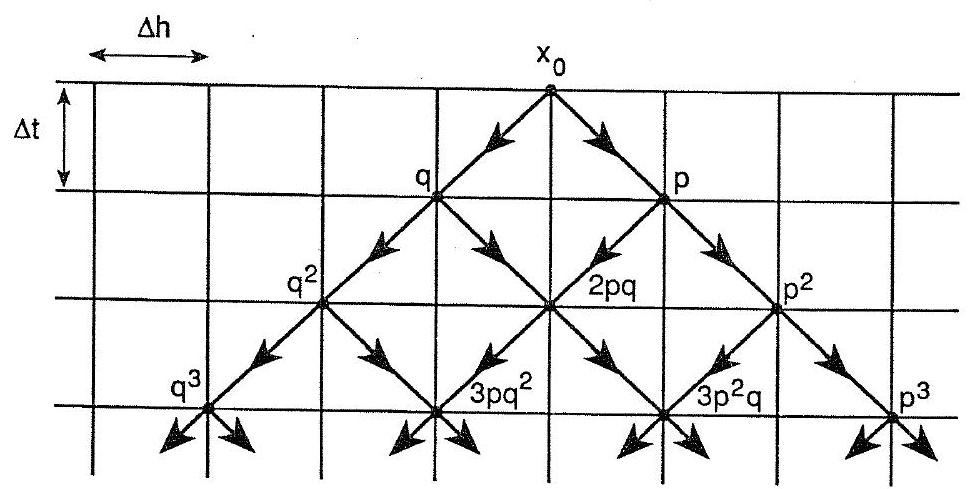
\includegraphics[max width=\textwidth]{2024_03_12_f639bb6397b3ab65b08bg-02}
    \caption{Random walk representation.}\label{fig: 1.1}
\end{figure}
A time interval of length $t$ has $n=t / \Delta t$ such discrete steps. Since the successive steps of the random walk are independent, the cumulated change $\left(x_{t}-x_{0}\right)$ is a binomial variate with mean
\begin{align*}
n(p-q) \Delta h=t(p-q) \Delta h / \Delta t
\end{align*}
and variance
\begin{align*}
4 n p q(\Delta h)^{2}=4 t p q(\Delta h)^{2} / \Delta t
\end{align*}
These expressions are minor modifications of the very familiar and elementary binomial distribution. There a `success' in any one trial counts as 1 and occurs with probability $p$, while a failure counts as 0 and occurs with probability $q=1-p$. The (random) number of successes in $n$ independent trials has expectation $n p$ and variance $n p q$. The expressions just above are perfectly analogous. Now success counts as $\Delta h$ and failure as $-\Delta h$; therefore for example the variance is $4(\Delta h)^{2}$ times that of the usual binomial expression.

Now set
\begin{align}
\Delta h=\sigma \sqrt{\Delta t} \label{1.4}
\end{align}
and
\begin{align}
p=\frac{1}{2}\left[1+\frac{\mu}{\sigma} \sqrt{\Delta t}\right], \quad q=\frac{1}{2}\left[1-\frac{\mu}{\sigma} \sqrt{\Delta t}\right] \label{1.5}
\end{align}
or
\begin{align*}
p=\frac{1}{2}\left[1+\frac{\mu}{\sigma^{2}} \Delta h\right], \quad q=\frac{1}{2}\left[1-\frac{\mu}{\sigma^{2}} \Delta h\right]
\end{align*}
Then
\begin{align*}
4 p q=1-\left(\frac{\mu}{\sigma}\right)^{2} \Delta t
\end{align*}
Substitute these into the above expressions, and let $\Delta t$ go to zero. For given $t$, the number of steps goes to infinity. Then the binomial distribution converges to the normal, with mean
\begin{align*}
t \frac{\mu}{\sigma^{2}} \Delta h \frac{\Delta h}{\Delta t}=\mu t
\end{align*}
and variance
\begin{align*}
t\left[1-\left(\frac{\mu}{\sigma}\right)^{2} \Delta t\right] \frac{\sigma^{2} \Delta t}{\Delta t} \rightarrow \sigma^{2} t
\end{align*}
These are exactly the values we need for Brownian motion. Thus we can regard Brownian motion as the limit of the random walk, when the time interval and the space step-length go to zero together, while preserving the relation (\ref{1.4}) between them.

The mean of $\left(x_{t}-x_{0}\right)$ is $\mu t$, and its standard deviation is $\sigma \sqrt{t}$. For large $t$, we have $\sqrt{t} \ll t$; in the long run, the trend is the dominant determinant of Brownian motion. But for small $t$, we have $t \ll \sqrt{t}$, so volatility dominates in the short run.

Another manifestation of this volatility is seen by calculating the expected length of a path. We have
\begin{align*}
E(|\Delta x|)=\Delta h
\end{align*}
so the total expected length of the path over the time interval from 0 to $t$ is
\begin{align*}
t \Delta h / \Delta t=t \sigma / \sqrt{\Delta t} \rightarrow \infty
\end{align*}
as $\Delta t$ goes to zero. For small but finite $\Delta t$, the total length of almost all sample paths is very large. Therefore each path must have many ups and downs and look very jagged. Most such sample paths are not differentiable. When discussing the expected rate of change, therefore, we must write $E[d x] / d t$, not $E[d x / d t]$.

\subsection{Itô's Lemma}
Suppose $x$ follows Brownian motion with parameters $(\mu, \sigma)$. Consider a stochastic process $y$ that is related to $x$ by $y=f(x)$ where $f$ is a given non-random function. We want to relate changes in $y$ to those in $x$. The rules of conventional calculus suggest writing $d y=f^{\prime}(x) d x$ and taking expectations. But this turns out to be wrong. Starting at $y_{0}=f\left(x_{0}\right)$, consider the position a small amount of time $t$ later.
\begin{align*}
y_{t}-y_{0}=f^{\prime}\left(x_{0}\right)\left(x_{t}-x_{0}\right)+\frac{1}{2} f^{\prime \prime}\left(x_{0}\right)\left(x_{t}-x_{0}\right)^{2}+\ldots
\end{align*}
Hence
\begin{align*}
\begin{aligned}
E\left[y_{t}-y_{0}\right] & =f^{\prime}\left(x_{0}\right) E\left[x_{t}-x_{0}\right]+\frac{1}{2} f^{\prime \prime}\left(x_{0}\right) E\left[\left(x_{t}-x_{0}\right)^{2}\right]+\ldots \\
& =f^{\prime}\left(x_{0}\right) \mu t+\frac{1}{2} f^{\prime \prime}\left(x_{0}\right)\left[\sigma^{2} t+\mu^{2} t^{2}\right]+\ldots \\
& =\left[\mu f^{\prime}\left(x_{0}\right)+\frac{1}{2} \sigma^{2} f^{\prime \prime}\left(x_{0}\right)\right] t+\ldots,
\end{aligned}
\end{align*}
where in each case the dots represent terms in higher powers of $t$ that can be ignored when $t$ is small. But note that the second order term in the Taylor expansion of $f(x)$ contributes a term that is of the first order in $t$. The reason is that the variance of the increments of $x$ is linear in $t$. This is the feature that makes the calculus of Brownian motion so different from the usual calculus of non-random variables.

A similar calculation will show that
\begin{align*}
\operatorname{Var}\left[y_{t}-y_{0}\right]=f^{\prime}\left(x_{0}\right)^{2} \sigma^{2} t+\ldots
\end{align*}
Let $x$ denote a general starting position and $y=f(x)$. Consider the infinitesimal increment $d y$ over the next infinitesimal time interval $dt$. We can use the above expressions replacing $t$ bt $dt$ and ignoring higher order terms in $dt$. Therefore $d y$ has mean
\begin{align*}
E[d y]=\left[f^{\prime}(x) \mu+\frac{1}{2} f^{\prime \prime}(x) \sigma^{2}\right] d t
\end{align*}
and variance
\begin{align*}
\operatorname{Var}[d y]=f^{\prime}(x)^{2} \sigma^{2} d t
\end{align*}
So $y$ follows the general diffusion process defined by
\begin{align}
d y=\left[f^{\prime}(x) \mu+\frac{1}{2} f^{\prime \prime}(x) \sigma^{2}\right] d t+f^{\prime}(x) \sigma d w . \label{1.6}
\end{align}

This is Itô's Lemma in the form that will prove most useful for us. A slight generalization is easily available: if $y=f(x, t)$, the Taylor expansion has an addition term in $f_{t}$, and
\begin{align}
d y=\left[f_{x}(x, t) \mu+\frac{1}{2} f_{x x}(x, t) \sigma^{2}+f_{t}(x, t)\right] d t+f_{x}(x, t) \sigma d w \label{1.7}
\end{align}

For a simple intuition, return to the discrete random walk formulation, and suppose $x$ has zero trend, so $p=q=1 / 2$. Now $E[\Delta x]=0$,
and as time passes the distribution of $x$ merely spreads out with linearly increasing variance around an unchanging mean. From the standard intuition of risk-aversion, or from Jensen's inequality, we know that the sign of $E[\Delta y]$ depends on the curvature of the function $f$. A riskaverter will dislike the increase in risk, and a risk-lover will like it Therefore $E[\Delta y]$ will be negative if $f$ is concave ( $f^{\prime \prime}$ is negative) and positive if $f$ is convex ( $f^{\prime \prime}$ is positive). Figure 1.2 shows the latter case. We have
\begin{align*}
\begin{aligned}
E[\Delta y]= & \frac{1}{2} f(x+\Delta h)+\frac{1}{2} f(x-\Delta h)-f(x) \\
= & \frac{1}{2}\left[f^{\prime}(x) \Delta h+\frac{1}{2} f^{\prime \prime}(x)(\Delta h)^{2}+\ldots\right] \\
& +\frac{1}{2}\left[-f^{\prime}(x) \Delta h+\frac{1}{2} f^{\prime \prime}(x)(\Delta h)^{2}+\ldots\right] \\
= & \frac{1}{2} f^{\prime \prime}(x)(\Delta h)^{2}+\ldots=\frac{1}{2} f^{\prime \prime}(x) \sigma^{2} \Delta t+\ldots
\end{aligned}
\end{align*}
Regarding $\Delta t$ as an infinitesimal $dt$, this is exactly the same as the additional term in (\ref{1.6}) that ordinary calculus would not have led us to expect. Thus Itô's Lemma is basically a consequence of Jensen's Inequality when we take into account the particular relation between the space steps and the time intervals of Brownian motion. Readers can now do the slightly messier case where $\mu \neq 0$ and get an exact correspondence with (1.6).

\subsection{Geometric Brownian motion}
Now suppose $x$ follows the Brownian motion (1.1), and let $X=e^{x}$. Itô’s Lemma gives
\begin{align*}
E[d X]=\left[e^{x} \mu+\frac{1}{2} e^{x} \sigma^{2}\right] d t=X\left[\mu+\frac{1}{2} \sigma^{2}\right] d t
\end{align*}
and
\begin{align*}
\operatorname{Var}[d X]=\left[e^{x}\right]^{2} \sigma^{2} d t=X^{2} \sigma^{2} d t
\end{align*}
Therefore the process of $X$ can be written
\begin{align*}
d X / X=\left[\mu+\frac{1}{2} \sigma^{2}\right] d t+\sigma d w .
\end{align*}
This is called a geometric or proportional Brownian motion. It is particularly useful in economics because it provides a good first approximation of the dynamics of exchange rates, prices of natural resources, and more generally many asset prices.
\begin{figure}
    \centering
    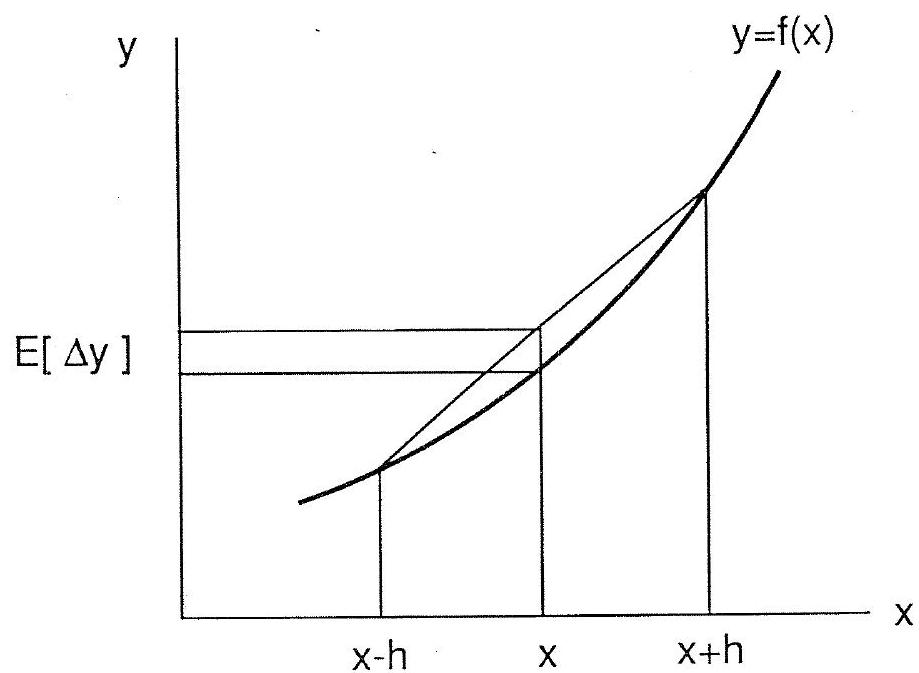
\includegraphics[max width=\textwidth]{2024_03_12_f639bb6397b3ab65b08bg-04}
    \caption{Itô's Lemma.}\label{fig: 1.2}
\end{figure}
Conversely, if $X$ follows the geometric Brownian motion
\begin{align}
d X / X=\nu d t+\sigma d z \label{1.8}
\end{align}
then using Itô's Lemma we find that $x=\ln X$ follows the ordinary or absolute Brownian motion
\begin{align*}
d x=\left[\nu-\frac{1}{2} \sigma^{2}\right] d t+\sigma dw
\end{align*}

We will often have occasion to use this correspondence between geometric and absolute Brownian motions in what follows. Note that when $x=\ln X$, the trend coefficients on the right hand sides of the expressions (\ref{1.1}) for $d x$ and (\ref{1.8}) for $d X / X$ differ by $\frac{1}{2} \sigma^{2}$. Thus $d \ln X \neq d X / X$; this is the Jensen-Itô effect discussed above. The logarithm is a concave function, and therefore $d \ln X<d X / X$, and a calculation shows that $\frac{1}{2} \sigma^{2} d t$ is just the right difference.

Suppose $X$ follows the geometric Brownian motion (1.8), starting at $t=0$ in the known position $X_{0}$. Let $x=\ln X$ and $x_{0}=\ln X_{0}$. We know that $x$ follows the absolute Brownian motion (\ref{1.1}) with $\mu=\nu-\frac{1}{2} \sigma^{2}$. Then at any positive time $t, x_{t}=\ln X_{t}$ is normally\\
distributed with mean $\left(x_{0}+\mu t\right)$ and variance $\sigma^{2} t$. In other words, $X_{t}$ has a lognormal distribution with parameters $\left(x_{0}+\mu t\right)$ and $\sigma \sqrt{t}$. For such a distribution, it can be shown that
\begin{align*}
E\left[X_{t}\right]=\exp \left(x_{0}+\mu t+\frac{1}{2} \sigma^{2} t\right)=X_{0} e^{\nu t}
\end{align*}
This is a special case of the formula for a general exponential. We see once again the Jensen-Itô effect at work; the exponential is a convex function, therefore
\begin{align*}
E\left[X_{t}\right]=E[\exp x]>\exp E\left[x_{t}\right]=\exp \left(x_{0}+\mu t\right)
\end{align*}

These repetitious details may seem boring, but they help fix the basics of the Itô calculus in the beginner's mind and thereby reduce the risk of many subsequent errors. Readers can get further practice by finding the stochastic process for $(1 / X)$ when $X$ follows the geometric Brownian motion (1.8). This is useful, for example, when converting formulas based on the dollar-yen exchange rate to ones using the yen-dollar rate.

\subsection{Some generalizations}
An obvious generalization of the Brownian motion (\ref{1.1}) is obtained by letting the trend coefficient $\mu$ and the volatility coefficient $\sigma$ depend on the current state $x$ and also on time; thus
\begin{align}
d x=\mu(x, t) d t+\sigma(x, t) d w . \label{1.9}
\end{align}
A process whose trend and volatility coefficients are functions of the current state is often called a diffusion process; when they are functions of time as well, it is sometimes called an Itô process.

The geometric Brownian motion of Section 1.3 is an important special case. We can cast (\ref{1.8}) in the diffusion process from (\ref{1.9}) by writing
\begin{align*}
d X=\mu X d t+\sigma X dw
\end{align*}
so the coefficients are both proportional to the current state.

In some economic applications, we need processes that revert toward some central level $\bar{x}$ of the state variable. For example, there may be an equilibrating force on prices. Now the trend coefficient has a sign opposite to that of $(x-\bar{x})$. When the mean reversion is linear, we have
\begin{align}
d x=-\theta(x-\bar{x}) d t+\sigma dw \label{1.10}
\end{align}
where $\theta$ is some positive constant.

Finally, several variables $x_{i}$ for $i=1,2, \ldots m$ may follow Brownian motion, their volatility components being linear combinations of independent standard Wiener processes $w_{j}$ for $j=1,2, \ldots n$ :
\begin{align*}
d x_{i}=\mu_{i} d t+\sum_{j=1}^{n} a_{i j} d w_{j}
\end{align*}
Then
\begin{align*}
E\left[d x_{i}\right]=\mu_{i} dt
\end{align*}
and
\begin{align*}
\operatorname{Var}\left[d x_{i}\right]=\sum_{j=1}^{n}\left(a_{i j}\right)^{2} d t, \quad \operatorname{Cov}\left[d x_{i}, d x_{k}\right]=\sum_{j=1}^{n} a_{i j} a_{k j} dt.
\end{align*}
This allows quite general correlation between the different $d x_{i}$. Such multi-variable processes are important in financial economics, but I will not develop these more advanced applications here.

\section{Discounted Present Values}
Here we consider an economic unit, such as a firm, in a dynamic stochastic setting. Its state at time $t$ is given by a state variable $x_{t}$ that follows a Brownian motion with exogenous parameters $\mu$ and $\sigma$. There is a net flow payoff $f\left(x_{t}\right)$, such as profit or dividend, that depends on the state $x_{t}$. The expected present value $F(x)$ of the payoff starting at a given initial position $x_{0}=x$, and using an exogenously specified discount rate $\rho$, is defined by
\begin{align}
F(x)=E\left\{\int_{0}^{\infty} f\left(x_{t}\right) e^{-\rho t} d t \mid x_{0}=x\right\} \label{2.1}
\end{align}
Ultimately, we will be interested in controlling or regulating the motion of $x_{t}$ to optimize such expected present values net of the cost of control. To this end, we begin by evaluating $F(x)$ explicitly when
$f(x)$ has some particularly simple functional forms such as exponentials and polynomials. Then we can get power series expressions for $F(x)$ when $f(x)$ is any analytic function.

\subsection{Present values for exponential and polynomials}
Here we consider the special case when the flow payoff has the form
\begin{align*}
f(x)=\exp (\lambda x)
\end{align*}
The discounted present value $F(x)$ will be finite when $\lambda$ is in a certain range, which will be found in course of the calculation.

Starting from the initial value $x_{0}=x$, the random position $x_{t}$ at time $t$ has a normal distribution with mean $(x+\mu t)$ and variance $\sigma^{2} t$. Then
\begin{align*}
E\left[\exp \left(\lambda x_{t}\right) \mid x_{0}=x\right]=\exp \left[\lambda(x+\mu t)+\frac{1}{2} \lambda^{2} \sigma^{2} t\right]
\end{align*}

Note the Jensen-Ito effect at work for the convex exponential function yet again.

Using this expectation, we have the present value
\begin{align}
F(x) & =\int_{0}^{\infty} E\left[\exp \left(\lambda x_{t}\right) \mid x_{0}=x\right] \exp (-\rho t) d t \\
& =\exp (\lambda x) \int_{0}^{\infty} \exp \left[-\left(\rho-\lambda \mu-\frac{1}{2} \lambda^{2} \sigma^{2}\right) t\right] d t \\
& =\exp (\lambda x) /\left(\rho-\lambda \mu-\frac{1}{2} \lambda^{2} \sigma^{2}\right)
\label{2.3}
\end{align}
The integral converges provided the denominator is positive.

Such a convergence condition will appear repeatedly in such calculations. Therefore it is useful to give it a uniform notation and interpretation at the outset. For this purpose, define the function
\begin{align}
\phi(\xi) \equiv \rho-\xi \mu-\frac{1}{2} \xi^{2} \sigma^{2} \label{2.4}
\end{align}

which I shall label the Fundamental Quadratic of Brownian motion. Let us examine its properties. Since the coefficient of the quadratic term is negative, $\phi(\xi)$ goes to $-\infty$ as $\xi$ goes to $\pm \infty$. We assume that the discount rate $\rho$ is positive, which is the natural economic condition to ensure a finite present value for a constant flow. With $\phi(0)=\rho>0$, the quadratic equation $\phi(\xi)=0$ has two real roots, one negative, say $-\alpha$, and the other positive, say $\beta$. Then $\phi(\xi)$ is positive when $\xi$ is in the interval $(-\alpha, \beta)$, and negative outside it. Figure 2.1 shows this graphically.
\begin{figure}
    \centering
    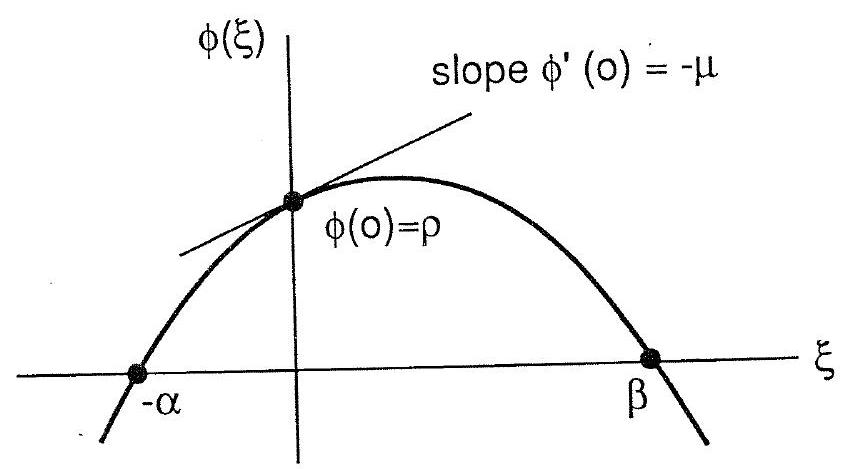
\includegraphics[max width=\textwidth]{2024_03_12_f639bb6397b3ab65b08bg-06}
    \caption{The Fundamental Quadratic.}
    \label{fig: 2.1}
\end{figure}

Thus the condition for the convergence of the integral in (\ref{2.3}) amounts to requiring that $\lambda$ lies in the interval $(-\alpha, \beta)$. This includes $\lambda=0$, a fact which will prove useful soon.

We can use the formula (\ref{2.3}) above to derive an expression for $F(x)$ when $f(x)$ is any integer power $x^{n}$. Begin by observing that for the exponential flow function,
\begin{align*}
F(x) & =E\left[\left.\int_{0}^{\infty} \sum_{n=0}^{\infty} \frac{1}{n !}\left(\lambda x_{t}\right)^{n} e^{-\rho t} d t \right\rvert\, x_{0}=x\right] \\
& =\sum_{n=0}^{\infty} \frac{\lambda^{n}}{n !} E\left[\int_{0}^{\infty} x_{t}^{n} e^{-\rho t} d t \mid x_{0}=x\right]
\end{align*}
Now we can expand the right hand side of (\ref{2.3}) in powers of $\lambda$. Since the resulting power series must equal the series just above for all $\lambda$ in a neighborhood that includes $\lambda=0$, we can equate the coefficients of $\lambda^{n}$ on the two sides. This yields an expression for the expected present value of the $n$th power of $x$.

To expand the right hand side of (2.3), note that
\begin{align*}
\exp (\lambda x)=\sum_{n=0}^{\infty} \frac{1}{n !} \lambda^{n} x^{n}
\end{align*}
and
\begin{align*}
\left[\rho-\mu \lambda-\frac{1}{2} \sigma^{2} \lambda^{2}\right]^{-1}=\frac{1}{\rho} \sum_{n=0}^{\infty} \rho^{-n}\left(\mu \lambda+\frac{1}{2} \sigma^{2} \lambda^{2}\right)^{n}
\end{align*}

For each $n$, the $n$th power of the sum of terms in $\lambda$ and $\lambda^{2}$ in the second of these series must be written out using the binomial theorem. Then the two series can be multiplied together and the coefficients of like powers of $\lambda$ collected to express the product as a single power series. This is tedious to do for higher powers, and in Section 2.5 we shall develop an alternative approach that is simpler. But the first few powers are not too hard, and yield the following results for the discounted present values of $x$ and $x^{2}$:
\begin{gather}
E \int_{0}^{\infty} x_{t} e^{-\rho t} d t=\frac{\mu}{\rho^{2}}+\frac{x}{\rho}, \label{2.5} \\
E \int_{0}^{\infty} x_{t}^{2} e^{-\rho t} d t=\left(\frac{\sigma^{2}}{\rho^{2}}+\frac{2 \mu^{2}}{\rho^{3}}\right)+\frac{2 \mu x}{\rho^{2}}+\frac{x^{2}}{\rho} . \label{2.6}
\end{gather}
This last expression will prove useful in the menu cost application of Section 4.5 below.

Finally, consider any analytic $f(x)$ with the power series representation
\begin{align*}
f(x)=\sum_{n=0}^{\infty} f_{n} x^{n}
\end{align*}
assumed uniformly convergent for all $x$. Having found the expected present values of all integer powers, we can integrate term by term to find the $F(x)$ corresponding to this analytic $f(x)$. Thus we can in principle complete the calculation of present values for most common functions of Brownian motion.

\subsection{Present values for powers of geometric Brownian motion}
Next suppose $X$ follows the geometric Brownian motion (1.8), namely
\begin{align*}
d X / X=\nu d t+\sigma dw.
\end{align*}
We want to find the expected present value when the flow payoff is $g(X)=X^{\lambda}$. Note that $x=\ln (X)$ follows the Brownian motion
\begin{align*}
d x=\left(\nu-\frac{1}{2} \sigma^{2}\right) dt+\sigma dw
\end{align*}
and $X^{\lambda}=\exp (\lambda x)$. Using (\ref{2.3}) for this, we have
\begin{align}
E\left\{\int_{0}^{\infty} X_{t}^{\lambda} e^{-\rho t} d t\right\} & =\exp (\lambda x) /\left[\rho-\left(\nu-\frac{1}{2} \sigma^{2}\right) \lambda-\frac{1}{2} \sigma^{2} \lambda^{2}\right] \\
& =X^{\lambda} /\left[\rho-\nu \lambda-\frac{1}{2} \sigma^{2} \lambda(\lambda-1)\right]
\label{2.7}
\end{align}
provided the integral converges, for which we need the denominator to be positive.

The convergence condition is now defined in terms of a slightly different quadratic
\begin{align}
\psi(\xi) \equiv \rho-\nu \xi-\frac{1}{2} \sigma^{2} \xi(\xi-1) \label{2.8}
\end{align}
I make two economically natural assumptions that help locate the roots: $\rho>0$, which ensures convergence of the expected present value of a constant flow, and $\rho>\nu$, which guarantees the convergence
of the expected present value of $X_{t}$ itself. Then the roots of the quadratic (\ref{2.8}) are $-\gamma<0$ and $\delta>1$. For convergence of (\ref{2.7}) we require that $\lambda$ should lie in the interval $(-\gamma, \delta)$.

Note that the expected present value is finite for all integer powers of absolute Brownian motion, but not for all those of geometric Brownian motion. The reason is that a power of geometric Brownian motion is like an exponential of absolute Brownian motion. Applying Itô's Lemma again, we find that $Y=X^{\lambda}$ follows the geometric Brownian motion
\begin{align*}
d Y / Y=\left[\lambda \nu+\frac{1}{2} \lambda(\lambda-1) \sigma^{2}\right] dt+\lambda \sigma dw
\end{align*}
For convergence of the expected present value of $Y$, the discount rate must exceed the trend growth rate of $Y$. Inspection shows this to be just the condition $\psi(\lambda)>0$.

Note also the relationship between the two fundamental quadratics, (\ref{2.4}) for an absolute Brownian motion $\left\{x_{t}\right\}$ with parameters $(\mu, \sigma)$ and (\ref{2.8}) for a geometric Brownian motion $\left\{X_{t}\right\}$ with parameters $(\nu, \sigma)$. If in fact $x=\ln (X)$, then the two trend parameters will be related to each other by $\mu=\nu-1 / 2 \sigma^{2}$. Substituting in (2.8), we will get
\begin{align*}
\psi(\xi) & =\rho-\left(\mu+\frac{1}{2} \sigma^{2}\right) \xi-\frac{1}{2} \sigma^{2} \xi(\xi-1) \\
& =\rho-\mu \xi-\frac{1}{2} \sigma^{2} \xi^{2}=\phi(\xi)
\end{align*}
and then the roots will also correspond, with $\alpha=\gamma$ and $\beta=\delta$.

\subsection{A basic differential equation for present value}
Let us return to the absolute Brownian motion $x$ and the flow payoff $f(x)$, and consider an alternative characterization of the expected present value $F(x)$ defined in (2.1). For this purpose, we split the integral into the contribution over the initial infinitesimal time interval from 0 to $dt$, and the integral from $dt$ to $\infty$. In spirit this is exactly like the decomposition of an intertemporal objective in dymanic programming; the only difference is that we have no control variables here. Now at time $dt$ the state variable will attain a value $(x+d x)$ that is not known at time 0 , although its distribution is. The integral from there on will be just $F(x+d x)$, which must be discounted back to time 0. Thus we have
\begin{align*}
F(x)=f(x) dt+e^{-\rho dt} E[F(x+dx)].
\end{align*}
Note that this is already an approximation in regarding $f(x)$ as constant over the small interval $dt$. The resulting error in $f(x) d t$ is of order $d t^{2}$, and therefore negligible in the limit as $dt$ goes to zero. We further simplify the expression, continuing to ignore terms that are small relative to $dt$.
\begin{align*}
F(x) & =f(x) d t+(1-\rho d t)(F(x)+\{E[F(x+d x)]-F(x)\}) \\
& =f(x) d t+F(x)-\rho F(x) d t+\{E[F(x+d x)]-F(x)\}
\end{align*}
Therefore
\begin{align}
\rho F(x) d t & =f(x) d t+\{E[F(x+d x)]-F(x)\} \\
& =f(x) d t+E[d F]
\label{2.9}
\end{align}
This is an arbitrage equation. Think of the entitlement to the flow payoffs as a capital asset; $F(x)$ is its value. Contemplate holding this asset over the period $(t, t+d t)$. This yields a dividend $f(x) d t$, and an expected capital gain $E[d F]$. The sum of these two should equal the normal return $\rho F(x) d t$.
By Itô's Lemma,
\begin{align*}
E[d F]=\mu F^{\prime}(x) dt+\frac{1}{2} \sigma^{2} F^{\prime \prime}(x) dt.
\end{align*}
Substituting into (\ref{2.9}) and dividing by $dt$, we get
\begin{align}
\frac{1}{2} \sigma^{2} F^{\prime \prime}(x)+\mu F^{\prime}(x)-\rho F(x)+f(x)=0 . \label{2.10}
\end{align}

\subsection{Derivation by discrete approximation}
We regarded Brownian motion as the limit of a discrete random walk, and we can also derive the differential equation (\ref{2.10}) by that approach. This may be easier for some readers to follow, and similar methods will prove useful in later sections where we consider controlling or regulating the motion. Therefore I present this derivation before turning to the solution of the equation.

Label the discrete points in the $x$ space by $i$, and the discrete time periods by $j$. Let $i_{j}$ denote the position of the particle at time $j$; future positions are of course random variables given our initial information at $j=0$. Then the expected present value can be written as
\begin{align*}
F(i)=E\left\{\sum_{j=0}^{\infty} f\left(i_{j}\right) \Delta t e^{-j \rho \Delta t} \mid i_{0}=i\right\}
\end{align*}
After the first step, the same problem restarts with a new initial state $i_{1}$, which from the time 0 perspective can be either $(i+1)$ with probability $p$ or $(i-1)$ with probability $q$. Thus the expectation on the right hand side becomes
\begin{align*}
F(i)=f(i) \Delta t+e^{-\rho \Delta t}[p F(i+1)+q F(i-1)]
\end{align*}
Now expand the right hand side, ignoring terms of higher order than $\Delta t$. Note that
\begin{align*}
e^{-\rho \Delta t}=1-\rho \Delta t+\ldots
\end{align*}
Next, using definition (1.5') of $p$ and $q$, and the relation (\ref{1.4}) between the stepsize $\Delta h$ and the time interval $\Delta t$, we get
\begin{align*}
p F(i+1)+q F(i-1)= & \frac{1}{2}[1+(\mu / \sigma) \sqrt{\Delta t}] F(x+\Delta h) \\
& +\frac{1}{2}[1-(\mu / \sigma) \sqrt{\Delta t}] F(x-\Delta h) \\
= & \frac{1}{2}[1+(\mu / \sigma) \sqrt{\Delta t}]\left[F(x)+F^{\prime}(x) \Delta h\right. \\
& \left.+\frac{1}{2} F^{\prime \prime}(x)(\Delta h)^{2}+\ldots\right] \\
& +\frac{1}{2}[1-(\mu / \sigma) \sqrt{\Delta t}][F(x) \\
& \left.-F^{\prime}(x) \Delta h+\frac{1}{2} F^{\prime \prime}(x)(\Delta h)^{2}+\ldots\right] \\
= & F(x)+\mu F^{\prime}(x) \Delta t+\frac{1}{2} \sigma^{2} F^{\prime \prime}(x) \Delta t+\ldots
\end{align*}
Substituting and simplifying yields the same equation as (\ref{2.10}) above.

\subsection{The general solution}
The differential equation (\ref{2.10}) is linear (in the dependent variable and its derivatives). Therefore its general solution is the sum of two parts: any solution of the equation as a whole (the particular integral) and the general solution of the homogeneous part of the equation with the term $f(x)$ omitted (the complementary function).

To find the complementary function, write the homogeneous part of the equation:
\begin{align*}
\frac{1}{2} \sigma^{2} F^{\prime \prime}(x)+\mu F^{\prime}(x)-\rho F(x)=0 .
\end{align*}
Its general solution can be expressed as a linear combination of two independent solutions. If we try solutions of the form $\exp (\xi x)$, we get
\begin{align*}
\exp (\xi \dot{x})\left[\frac{1}{2} \sigma^{2} \xi^{2}+\mu \xi-\rho\right]=0
\end{align*}
Since the exponential is always positive, this holds if and only if
\begin{align*}
\rho-\mu \xi-\frac{1}{2} \sigma^{2} \xi^{2}=0
\end{align*}
This is just the fundamental quadratic $\phi(\xi)$ introduced in (\ref{2.4}) above. So $\xi$ must equal $-\alpha$ or $\beta$, the two roots. The two roots are distinct, since $\rho>0$ ensures that the roots have opposite signs. Therefore the two solutions $e^{-\alpha x}$ and $e^{\beta x}$ are independent, and the general solution is
\begin{align}
A e^{-\alpha x}+B e^{\beta x}, \label{2.11}
\end{align}
where $A$ and $B$ are undetermined constants.

Finding a particular solution to the full equation (\ref{2.10}) is often an art, but for the exponential and polynomial forms we tried before, there are obvious choices.

Begin with the exponential case. When $f(x)=\exp (\lambda x)$, the form $F(x)=K \exp (\lambda x)$ suggests itself. Substituting in (2.10), we have
\begin{align*}
K\left(\frac{1}{2} \sigma^{2} \lambda^{2}+\mu \lambda-\rho\right) \exp (\lambda x)+\exp (\lambda x)=0
\end{align*}
or
\begin{align*}
K=-1 /\left(\frac{1}{2} \sigma^{2} \lambda^{2}+\mu \lambda-\rho\right)=1 / \phi(\lambda)
\end{align*}
using the notation of our fundamental quadratic (2.4). When $\lambda$ lies between the two roots $-\alpha$ and $\beta$ of the quadratic, $\phi(\lambda)$ is positive. Then $K$ is also positive.

Combining this particular solution and the earlier complementary function (2.11), the general solution for the expected present value in the exponential case becomes
\begin{align}
F(x)=\frac{1}{\phi(\lambda)} e^{\lambda x}+A e^{-\alpha x}+B e^{\beta x} \label{2.12}
\end{align}
where the constants $A$ and $B$ remain to be determined.

In fact a simple argument based on the definition (\ref{2.1}) shows that when the flow $f(x)$ is the exponential $\exp (\lambda x)$, the expected present values $F(x)$ must be a multiple of $\exp (\lambda x)$. To prove this, consider $F(x+h)$ for any $h$. This means the initial point of the process $x_{t}$ is now taken as $x_{0}=x+h$. For each path of the Brownian particle starting at $x$, there is an equiprobable parallel path starting at $x+h$.

Along the latter path, the flow is always $\exp (\lambda h)$ times that along the former. Then the same must hold for the expected present values. In particular,
\begin{align*}
F(h)=e^{\lambda h} F(0)
\end{align*}
To give a somewhat more formal argument, define $y_{t}=x_{t}-h$, and consider the stochastic process $y_{t}$. This is also a Brownian motion with
\begin{align*}
d y=d x=\mu dt+\sigma dw
\end{align*}
and the initial position $y_{0}=(x+h)-h=x$. The flow benefit can be written
\begin{align*}
f\left(x_{t}\right)=e^{\lambda x_{t}}=e^{\lambda h} e^{\lambda y_{t}}=e^{\lambda h} f\left(y_{t}\right).
\end{align*}
Integrating over time and taking expectations, we get
\begin{align*}
F(x+h) & =e^{\lambda h} E\left\{\int_{0}^{\infty} f\left(y_{t}\right) e^{-\rho t} d t \mid y_{0}=x\right\} \\
& =e^{\lambda h} F(x)
\end{align*}
Subtracting $F(x)$ from both sides, dividing by $h$, and letting $h$ go to zero, we get
\begin{align*}
\lim _{h \rightarrow 0} \frac{F(x+h)-F(x)}{h}=\lim _{h \rightarrow 0} \frac{\exp (\lambda h)-1}{h} F(x),
\end{align*}
or
\begin{align*}
F^{\prime}(x)=\lambda F(x).
\end{align*}
Then $F(x)$ must take the form $K \exp (\lambda x)$ where $K$ is a constant.

The general solution (\ref{2.12}) above was a combination of three terms, of which only the first, corresponding to the particular solution we guessed initially, had the right exponential form. Thus that guess is in fact the full solution, and both constants $A$ and $B$ in the complementary function (\ref{2.11}) are zero.

In the same way we will be able to guess the right solution as our particular integral for many simple forms of the flow function. The complementary function will play a more important role in the next section, where it will capture the modification to expected present values that is caused by the barriers. 

Next consider the polynomial case. When $f(x)=x^{n}$ for a positive integer $n$, a natural guess for the particular integral is
\begin{align}
F(x)=\sum_{m=0}^{n} a_{m} x^{m} \label{2.13}
\end{align}
Substituting this in (2.10), we get
\begin{align*}
\frac{1}{2} \sigma^{2} \sum_{m=2}^{n} m(m-1) a_{m} x^{m-2} & +\mu \sum_{m=1}^{n} m a_{m} x^{m-1} \\
& -\rho \sum_{m=0}^{n} a_{m} x^{m}+x^{n}=0
\end{align*}

Collecting like powers of $x$ together, and equating the coefficient of each separately to zero since the equation must hold as an identity in $x$, we find
\begin{align*}
a_{n}=1 / \rho, \quad a_{n-1}=n \mu / \rho^{2}
\end{align*}
and for $m=0,1,2, \ldots(n-2)$, the recursive relation
\begin{align}
\rho a_{m}=(m+1) \mu a_{m+1}+\frac{1}{2}(m+1)(m+2) \sigma^{2} a_{m+2}. \label{2.14}
\end{align}
This determines all the coefficients $a_{m}$. Once again we can verify that the expected present value cannot have any contribution from the exponentials of the complementary function (2.11), and therefore (\ref{2.13}) is the full solution. This method, while needing a recursive solution, is simpler than the power series expansion we developed in Section 2.1 above. Readers can explicity write out the results using the above recursion for $n=1$ and $n=2$, and check their consistency with the formulas (\ref{2.5}) and (\ref{2.6}) derived above by the power series method.

\subsection{Differential equation for geometric Brownian motion}
Now suppose the underlying variable is $X$, and it follows the proportional or geometric Brownian motion (1.8). Given a flow cost function $g(X)$, we want to find
\begin{align}
G(X)=E\left\{\int_{0}^{\infty} g\left(X_{t}\right) e^{-\rho t} d t \mid X_{0}=X\right\} \label{2.15}
\end{align}
Proceeding exactly as before, we get the arbitrage equation
\begin{align*}
\rho G(X) d t=g(X) dt+E[dG]
\end{align*}
and Itô's Lemma gives
\begin{align*}
E[dG]=\nu X G^{\prime}(X) dt+\frac{1}{2}(\sigma X)^{2} G^{\prime \prime}(X) dt
\end{align*}
Therefore the basic differential equation for the case of geometric Brownian motion is
\begin{align}
\frac{1}{2} \sigma^{2} X^{2} G^{\prime \prime}(X)+\nu X G^{\prime}(X)-\rho G(X)+g(X)=0 \label{2.16}
\end{align}
The complementary function (the general solution of the homogeneous part) of (\ref{2.16}) is easily seen to be
\begin{align}
C X^{-\gamma}+D X^{\delta} \label{2.17}
\end{align}
where $-\gamma$ and $\delta$ are the roots of the fundamental quadratic (\ref{2.8}) for geometric Brownian, and $C, D$ are constants to be determined.

Once again the particular integral must be guessed. In Section 2.2 above we considered a flow function of the form $g(X)=X^{\lambda}$. Using the differential equation method, the natural guess for the corresponding expected present value $G(X)$ is $K X^{\lambda}$ where $K$ is a constant to be determined. Substituting in (\ref{2.16}) we find
\begin{align*}
K\left[\frac{1}{2} \sigma^{2} \lambda(\lambda-1)+\nu \lambda-\rho\right] X^{\lambda}+X^{\lambda}=0,
\end{align*}
or
\begin{align*}
K=-1 /\left[\frac{1}{2} \sigma^{2} \lambda(\lambda-1)+\nu \lambda-\rho\right]=1 / \psi(\lambda),
\end{align*}
where $\psi(\lambda)$ is the fundamental quadratic for the geometric case, and is positive when $\lambda$ lies between the two roots $-\lambda$ and $\delta$.

An argument similar to that we made above in Section 2.5 for the case of absolute Brownian motion and an exponential flow shows in the present case that $G(X)$ must take the form $K X^{\lambda}$, in other words it inherits the homogeneity of degree $\lambda$ from $g(X)$. Then the full solution is just the particular integral we guessed; the constants $C$ and $D$ in the complementary function (\ref{2.17}) are both zero.

We can change variables to transform geometric Brownian motion into an absolute one, and this gives an alternative way to find expected present values. Define $x=\ln (X)$, which then follows the absolute Brownian motion (\ref{1.1}) with $\mu=\nu-\frac{1}{2} \sigma^{2}$. Now let $f(x)=g\left(e^{x}\right)$, use the earlier (\ref{2.1}) to get $F(x)$, and then set $G(X)=F(\ln (X))$. Let us check that the transformation yields the same ultimate result as the direct analysis of geometric Brownian motion above. Note that $F(x)=G\left(e^{x}\right)$, so
\begin{align*}
F^{\prime}(x)=e^{x} G^{\prime}\left(e^{x}\right)=X G^{\prime}(X)
\end{align*}
and
\begin{align*}
F^{\prime \prime}(x)=\left(e^{x}\right)^{2} G^{\prime \prime}\left(e^{x}\right)+e^{x} G^{\prime}\left(e^{x}\right)=X^{2} G^{\prime \prime}(X)+X G^{\prime}(X)
\end{align*}
Substituting in (2.10), we find
\begin{align*}
0 & =\frac{1}{2} \sigma^{2}\left[X^{2} G^{\prime \prime}(X)+X G^{\prime}(X)\right]+\mu X G^{\prime}(X)-\rho G(X)+g(X) \\
& =\frac{1}{2} \sigma^{2} X^{2} G^{\prime \prime}(X)+\left[\mu+\frac{1}{2} \sigma^{2}\right] X G^{\prime}(X)-\rho G(X)+g(X) \\
& =\frac{1}{2} \sigma^{2} X^{2} G^{\prime \prime}(X)+\nu X G^{\prime}(X)-\rho G(X)+g(X)
\end{align*}
which is just (2.16). Thus the two approaches are mutually consistent. And the transformation of the differential operators casts a new light on the nonlinearity leading to Itô's Lemma from a somewhat different angle.

\subsection{General diffusion processes}
If $x$ follows the general diffusion process (\ref{1.9}) rather than the simple Brownian motion (1.1), the expected value function $F(x)$ and the flow function $f(x)$ are linked by a differential equation that is a natural generalization of (2.10), namely
\begin{align}
\frac{1}{2} \sigma(x)^{2} F^{\prime \prime}(x)+\mu(x) F^{\prime}(x)-\rho F(x)+f(x)=0 . \label{2.18}
\end{align}
Unfortunately, the solution of this is not the corresponding simple generalization of the solution of (2.10). The complementary function is specific to each case depending on the functional forms of $\mu(x)$ and $\sigma(x)$, and does not have any simple form like (2.11). Analytical solution is possible only in very special cases. The geometric case was discussed above. for the linearly mean-reverting motion (1.10), a power series solution related to the Confluent Hypergeometric Function is available; an example is developed in Section 5.1 below. But many other applications require numerical solution of the differential equation.

If $x$ follows the Itô process (\ref{1.9}) whose parameters depend on time as well as the state $x$, or if the flow payoff is a function $f(x, t)$ likewise, or the process ends at a given time $T$ so the time remaining\\
to the end of the horizon matters, then we must allow the expected present value to depend on time too. Applying Itô's Lemma to $F(x, t)$ introduces an additional term for the time derivative as in (1.7), and then the basic equation becomes a partial differential equation
\begin{align}
\frac{1}{2} \sigma(x, t)^{2} F_{x x}(x, t) & +\mu(x, t) F_{x}(x, t)-\rho F(x, t)+F_{t}(x, t) \\
& +f(x, t)=0
\label{2.19}
\end{align}
The solution of this is much harder, and typically needs numerical methods.

\end{document}